\documentclass[aspectratio=169,10pt]{beamer}

\usetheme{Madrid}
\usecolortheme{seahorse}
\setbeamertemplate{navigation symbols}{}
\setbeamertemplate{caption}[numbered]
\setbeamertemplate{footline}{}

\usepackage[T1]{fontenc}
\usepackage[utf8]{inputenc}
\usepackage{amsmath,amssymb}
\usepackage{booktabs}
\usepackage{array}
\usepackage{tikz}
\usepackage{pgfplots}
\usepackage{xcolor}
\usepackage{hyperref}

\pgfplotsset{compat=1.18}
\usetikzlibrary{arrows.meta,positioning,shapes.geometric,fit,calc}

\definecolor{bankgreen}{HTML}{0F6B51}
\definecolor{bankgreen2}{HTML}{0F8B63}
\definecolor{bankred}{HTML}{B42318}
\definecolor{bankgold}{HTML}{B7892B}
\definecolor{softgreen}{HTML}{EAF6EF}
\definecolor{softred}{HTML}{FFF1F0}
\definecolor{ink}{HTML}{16211B}

\setbeamercolor{title}{fg=bankgreen}
\setbeamercolor{frametitle}{fg=bankgreen}
\setbeamercolor{structure}{fg=bankgreen}
\setbeamercolor{block title}{bg=bankgreen,fg=white}
\setbeamercolor{block body}{bg=softgreen,fg=ink}

\newcommand{\targetAUPRC}{0.70}
\newcommand{\targetAUROC}{0.90}
\newcommand{\targetFone}{0.70}
\newcommand{\bestAUPRC}{0.7593}
\newcommand{\bestAUROC}{0.9525}
\newcommand{\bestFone}{0.7303}
\newcommand{\bestThreshold}{0.9829}

\title[Federated Fraud Detection]{Federated Fraud Detection}
\subtitle{Privacy-Preserving IEEE-CIS Fraud Detection with Flower, PyTorch, FastAPI, and React}
\author{Presenter A \and Presenter B}
\institute{Distributed Systems Project}
\date{\today}

\begin{document}

\begin{frame}
  \titlepage
\end{frame}

\begin{frame}{Presentation Roadmap}
  \begin{columns}[T]
    \begin{column}{0.48\textwidth}
      \textbf{Presenter A}
      \begin{enumerate}
        \item Problem statement
        \item Dataset and client split
        \item Feature engineering
        \item Model and metrics
      \end{enumerate}
    \end{column}
    \begin{column}{0.48\textwidth}
      \textbf{Presenter B}
      \begin{enumerate}
        \item Federated architecture
        \item Training and aggregation
        \item Fault tolerance and scalability
        \item Live GUI demo and Q\&A
      \end{enumerate}
    \end{column}
  \end{columns}
  \vspace{0.4cm}
  \begin{block}{Goal}
    Prove that the project is a real distributed federated learning system with measurable fraud detection quality, recovery behavior, and a working inference demo.
  \end{block}
\end{frame}

\section{Problem and Dataset}

\begin{frame}{Problem Statement}
  \begin{block}{Main Problem}
    Fraud data is sensitive, imbalanced, and naturally distributed across clients, regions, or institutions.
  \end{block}
  \begin{columns}[T]
    \begin{column}{0.48\textwidth}
      \textbf{Centralized training risk}
      \begin{itemize}
        \item Raw transaction data must be moved to one place.
        \item Privacy and compliance risks increase.
        \item A single central dataset may not represent all clients equally.
      \end{itemize}
    \end{column}
    \begin{column}{0.48\textwidth}
      \textbf{Federated training idea}
      \begin{itemize}
        \item Each client keeps raw rows local.
        \item Clients send model updates and metrics.
        \item Server aggregates a shared fraud model.
      \end{itemize}
    \end{column}
  \end{columns}
\end{frame}

\begin{frame}{Dataset Summary}
  \begin{columns}[T]
    \begin{column}{0.50\textwidth}
      \begin{table}
        \centering
        \begin{tabular}{lr}
          \toprule
          Item & Value \\
          \midrule
          Dataset & IEEE-CIS Fraud Detection \\
          Rows & 590,540 \\
          Engineered features & 316 \\
          Fraud rows & 20,663 \\
          Fraud rate & 3.50\% \\
          Clients & 3 temporal clients \\
          \bottomrule
        \end{tabular}
      \end{table}
    \end{column}
    \begin{column}{0.45\textwidth}
      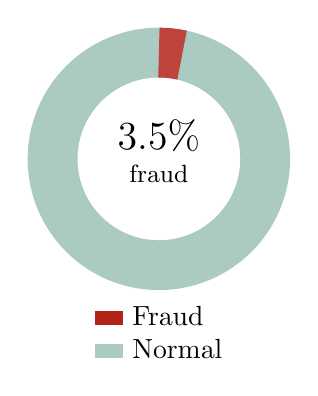
\begin{tikzpicture}
        \draw[line width=18pt, bankgreen!35] (0,0) circle (1.35);
        \draw[line width=18pt, bankred!85] (0,0) ++(90:1.35) arc[start angle=90,end angle=77.4,radius=1.35];
        \node[align=center] at (0,0.1) {\Large 3.5\%\\\small fraud};
        \node[align=left] at (0,-2.2) {\textcolor{bankred}{\rule{0.35cm}{0.18cm}} Fraud\\
          \textcolor{bankgreen!35}{\rule{0.35cm}{0.18cm}} Normal};
      \end{tikzpicture}
      \vspace{-0.2cm}
      \begin{block}{Why accuracy is misleading}
        A model can predict ``normal'' almost always and still appear accurate.
      \end{block}
    \end{column}
  \end{columns}
\end{frame}

\begin{frame}{Temporal Federated Client Split}
  \begin{columns}[T]
    \begin{column}{0.52\textwidth}
      \begin{table}
        \centering
        \begin{tabular}{lrrr}
          \toprule
          Client & Rows & Fraud rows & Fraud rate \\
          \midrule
          Client 0 & 196,846 & 5,835 & 2.96\% \\
          Client 1 & 196,847 & 7,745 & 3.93\% \\
          Client 2 & 196,847 & 7,083 & 3.60\% \\
          \bottomrule
        \end{tabular}
      \end{table}
    \end{column}
    \begin{column}{0.45\textwidth}
      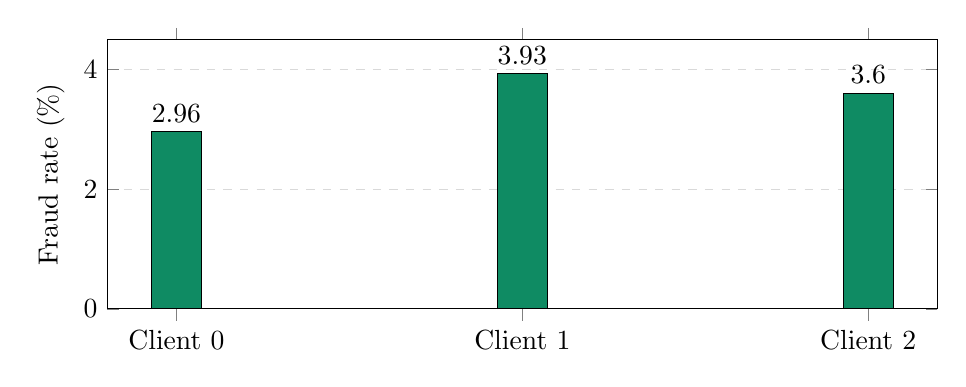
\begin{tikzpicture}
        \begin{axis}[
          ybar,
          width=\textwidth,
          height=5cm,
          ymin=0,
          ymax=4.5,
          ylabel={Fraud rate (\%)},
          symbolic x coords={Client 0,Client 1,Client 2},
          xtick=data,
          nodes near coords,
          nodes near coords align={vertical},
          bar width=18pt,
          ymajorgrids=true,
          grid style={dashed,gray!30}
        ]
          \addplot[fill=bankgreen2] coordinates {(Client 0,2.96) (Client 1,3.93) (Client 2,3.60)};
        \end{axis}
      \end{tikzpicture}
    \end{column}
  \end{columns}
  \begin{block}{Why temporal split}
    Fraud is time-dependent. Temporal split avoids future leakage and is closer to real deployment.
  \end{block}
\end{frame}

\section{Feature Engineering}

\begin{frame}{Data Pipeline Flow}
  \centering
  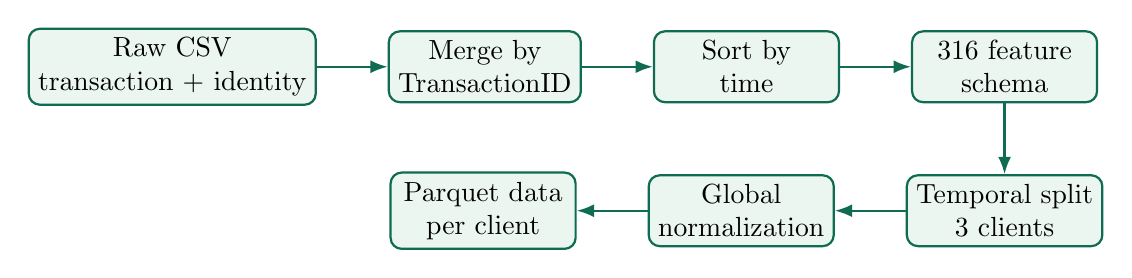
\begin{tikzpicture}[
    node distance=0.9cm,
    box/.style={rectangle, rounded corners, draw=bankgreen, fill=softgreen, thick, align=center, minimum width=2.35cm, minimum height=0.85cm},
    arrow/.style={-{Latex[length=2.2mm]}, thick, draw=bankgreen}
  ]
    \node[box] (raw) {Raw CSV\\transaction + identity};
    \node[box, right=of raw] (merge) {Merge by\\TransactionID};
    \node[box, right=of merge] (sort) {Sort by\\time};
    \node[box, right=of sort] (features) {316 feature\\schema};
    \node[box, below=of features] (split) {Temporal split\\3 clients};
    \node[box, left=of split] (norm) {Global\\normalization};
    \node[box, left=of norm] (parquet) {Parquet data\\per client};
    \draw[arrow] (raw) -- (merge);
    \draw[arrow] (merge) -- (sort);
    \draw[arrow] (sort) -- (features);
    \draw[arrow] (features) -- (split);
    \draw[arrow] (split) -- (norm);
    \draw[arrow] (norm) -- (parquet);
  \end{tikzpicture}
  \vspace{0.3cm}
  \begin{block}{Schema Contract}
    The GUI and API reconstruct the same feature order used during training.
  \end{block}
\end{frame}

\begin{frame}{Feature Groups}
  \begin{columns}[T]
    \begin{column}{0.50\textwidth}
      \begin{enumerate}
        \item Amount, transaction count, and volume
        \item Time: hour, day, risky-hour flag
        \item Product, card, email, device context
        \item Frequency encodings for repeated identities
        \item Backward-looking history for card, email, address, device, and pairs
      \end{enumerate}
    \end{column}
    \begin{column}{0.48\textwidth}
      \begin{block}{Presentation Line}
        Fraud is not detected from one field alone. The model learns patterns from amount, time, identity, velocity, and history signals together.
      \end{block}
    \end{column}
  \end{columns}
\end{frame}

\begin{frame}{Important Feature Formulas}
  \begin{columns}[T]
    \begin{column}{0.56\textwidth}
      \begin{align*}
        x_{\text{amount}} &= \log(1 + \text{TransactionAmt}) \\
        x_{\text{count,1h}} &= \log(1 + C_1) \\
        x_{\text{volume,1h}} &= \log(1 + \text{TransactionAmt} \cdot C_1) \\
        \text{distance}_{km} &= \text{dist1} \cdot 1.60934 \\
        x_{\text{velocity}} &= \log(1 + \operatorname{clip}(\text{velocity}_{kmh},0,2000)) \\
        \text{amt/txn} &= \log(1+\text{amount}) - \log(1+\text{count}+0.1)
      \end{align*}
    \end{column}
    \begin{column}{0.42\textwidth}
      \footnotesize
      \begin{itemize}
        \item \textbf{TransactionAmt}: raw purchase amount
        \item \(C_1\): IEEE-CIS count feature (recent transactions for the identity)
        \item \textbf{dist1}: raw distance field in the dataset
        \item \(\text{velocity}_{kmh}\): distance over time between transactions
        \item \(\operatorname{clip}(\cdot,0,2000)\): caps outlier speeds at 2000 km/h
      \end{itemize}
    \end{column}
  \end{columns}
  \begin{block}{Why log transforms}
    Fraud data has heavy-tailed amounts and counts. Log transforms reduce extreme scale while preserving ordering.
  \end{block}
\end{frame}

\begin{frame}{Backward-Looking History Formula}
  \begin{block}{Smoothed historical fraud rate}
    \[
      \operatorname{hist\_fraud\_rate}_{e}(t)
      =
      \frac{\operatorname{prev\_fraud}_{e}(t) + 32 \cdot \operatorname{global\_prior}(t)}
           {n_e(t) + 32}
    \]
  \end{block}
  \begin{columns}[T]
    \begin{column}{0.48\textwidth}
      \textbf{Symbols}
      \begin{itemize}
        \item \(e\): card, email, address, device, or pair
        \item \(\operatorname{prev\_fraud}_e(t)\): fraud count for \(e\) before \(t\)
        \item \(n_e(t)\): transaction count for \(e\) before \(t\)
        \item \(\operatorname{global\_prior}(t)\): dataset-wide fraud rate before \(t\)
      \end{itemize}
    \end{column}
    \begin{column}{0.48\textwidth}
      \textbf{Why smoothing}
      \begin{itemize}
        \item New identities have little history.
        \item The \(32\) term pulls small histories toward global fraud rate.
        \item As history grows, entity history dominates.
      \end{itemize}
    \end{column}
  \end{columns}
\end{frame}

\begin{frame}{Federated Normalization}
  Each client sends sufficient statistics, not raw rows:
  \[
    n_i,\quad s_{i,j}=\sum x_{i,j},\quad ss_{i,j}=\sum x_{i,j}^2
  \]
  Global feature mean:
  \[
    \mu_j = \frac{\sum_i s_{i,j}}{\sum_i n_i}
  \]
  Global standard deviation:
  \[
    \sigma_j =
    \sqrt{
      \frac{\sum_i ss_{i,j}}{\sum_i n_i}
      - \mu_j^2
    }
  \]
  Normalized feature:
  \[
    z_j = \frac{x_j - \mu_j}{\max(\sigma_j,10^{-8})}
  \]
  \begin{block}{Symbols}
    \footnotesize
    \(n_i\): row count at client \(i\) \quad
    \(s_{i,j},\,ss_{i,j}\): sum and sum-of-squares of feature \(j\) at client \(i\) \quad
    \(\mu_j,\sigma_j\): global mean/std of feature \(j\) \quad
    \(z_j\): normalized value used by the model
  \end{block}
\end{frame}

\section{Model and Metrics}

\begin{frame}{Model Architecture}
  \centering
  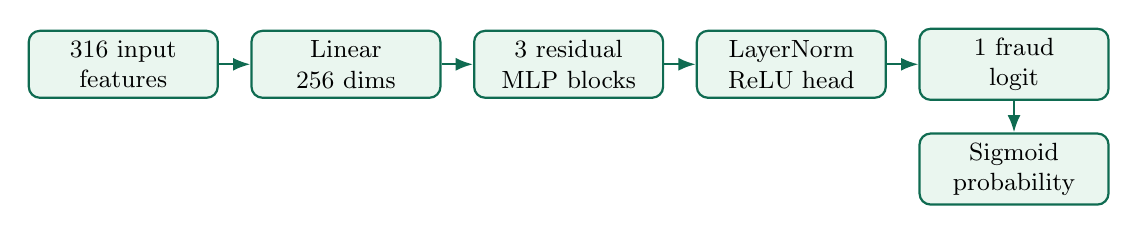
\begin{tikzpicture}[
    node distance=0.4cm,
    box/.style={rectangle, rounded corners, draw=bankgreen, fill=softgreen, thick, align=center, minimum width=2.4cm, minimum height=0.85cm, font=\small},
    arrow/.style={-{Latex[length=2.2mm]}, thick, draw=bankgreen}
  ]
    \node[box] (input) {316 input\\features};
    \node[box, right=of input] (proj) {Linear\\256 dims};
    \node[box, right=of proj] (res) {3 residual\\MLP blocks};
    \node[box, right=of res] (head) {LayerNorm\\ReLU head};
    \node[box, right=of head] (logit) {1 fraud\\logit};
    \node[box, below=of logit] (sig) {Sigmoid\\probability};
    \draw[arrow] (input) -- (proj);
    \draw[arrow] (proj) -- (res);
    \draw[arrow] (res) -- (head);
    \draw[arrow] (head) -- (logit);
    \draw[arrow] (logit) -- (sig);
  \end{tikzpicture}
  \vspace{0.4cm}
  \[
    p = \sigma(z) = \frac{1}{1 + e^{-z}}
  \]
  \footnotesize \(z\): the network's raw fraud logit \quad \(\sigma\): sigmoid, squashes \(z\) into a probability \(p \in (0,1)\)
\end{frame}

\begin{frame}{Decision Threshold}
  \begin{block}{Important demo point}
    The GUI does not use a naive threshold of \(0.5\). It uses the selected checkpoint's F1-optimized threshold.
  \end{block}
  \[
    \hat{y} =
    \begin{cases}
      1 & \text{if } p \geq \tau \\
      0 & \text{if } p < \tau
    \end{cases}
    \qquad
    \tau \approx \bestThreshold
  \]
  \footnotesize \(p\): model's predicted fraud probability \quad \(\tau\): decision threshold \quad \(\hat{y}\): final flag (1 = block/review, 0 = approve)
  \normalsize
  \begin{columns}[T]
    \begin{column}{0.48\textwidth}
      \textbf{Reliable preset}\\
      Low score, below threshold, decision: approve.
    \end{column}
    \begin{column}{0.48\textwidth}
      \textbf{Suspicious preset}\\
      High score, above threshold, decision: block or review.
    \end{column}
  \end{columns}
\end{frame}

\begin{frame}{Metrics: Confusion Matrix Terms}
  \begin{columns}[T]
    \begin{column}{0.46\textwidth}
      \centering
      \begin{tabular}{c|cc}
        & Predicted fraud & Predicted normal \\
        \hline
        Real fraud & TP & FN \\
        Real normal & FP & TN \\
      \end{tabular}
    \end{column}
    \begin{column}{0.50\textwidth}
      \begin{itemize}
        \item \textbf{TP}: fraud correctly flagged.
        \item \textbf{FP}: normal transaction incorrectly flagged.
        \item \textbf{FN}: fraud transaction missed.
        \item \textbf{TN}: normal transaction correctly approved.
      \end{itemize}
    \end{column}
  \end{columns}
  \begin{block}{Why this matters}
    Fraud detection must avoid both missed fraud and too many false alarms.
  \end{block}
\end{frame}

\begin{frame}{Metrics: Precision, Recall, and F1}
  \begin{columns}[T]
    \begin{column}{0.48\textwidth}
      \[
        \text{Precision}=\frac{TP}{TP+FP}
      \]
      \small
      When the system says ``fraud'', how often is it correct? High precision means fewer legitimate customers are incorrectly blocked.
      \vspace{0.4cm}
      \[
        \text{Recall}=\frac{TP}{TP+FN}
      \]
      \small
      Of all real fraud, how much did we catch? High recall means fewer fraud cases are missed.
    \end{column}
    \begin{column}{0.48\textwidth}
      \[
        F1 =
        \frac{2 \cdot \text{Precision} \cdot \text{Recall}}
             {\text{Precision}+\text{Recall}}
      \]
      \small
      F1 balances false alarms and missed fraud at one selected threshold.
      \vspace{0.35cm}
      \begin{block}{Demo link}
        The GUI uses the checkpoint's F1-optimized threshold, not a fixed \(0.5\).
      \end{block}
    \end{column}
  \end{columns}
\end{frame}

\begin{frame}{Metrics: AUPRC and AUROC}
  \begin{columns}[T]
    \begin{column}{0.48\textwidth}
      \begin{block}{AUPRC}
        Area under the precision-recall curve. It focuses on the rare fraud class and is stricter when only 3.5\% of rows are fraud.
      \end{block}
      \small
      Good AUPRC means high-scored transactions are often real fraud and real fraud appears near the top of the ranked list.
    \end{column}
    \begin{column}{0.48\textwidth}
      \begin{block}{AUROC}
        Area under the ROC curve. It measures broad ranking separation between fraud and normal transactions.
      \end{block}
      \small
      Simple explanation: randomly pick one fraud and one normal transaction; AUROC estimates how often fraud receives the higher score.
    \end{column}
  \end{columns}
  \vspace{0.25cm}
  \begin{block}{Demo link}
    If the suspicious preset scores much higher than the reliable preset, the model is showing the ranking behavior rewarded by AUPRC and AUROC.
  \end{block}
\end{frame}

\section{Federated Learning Architecture}

\begin{frame}{Federated System Architecture}
  \centering
  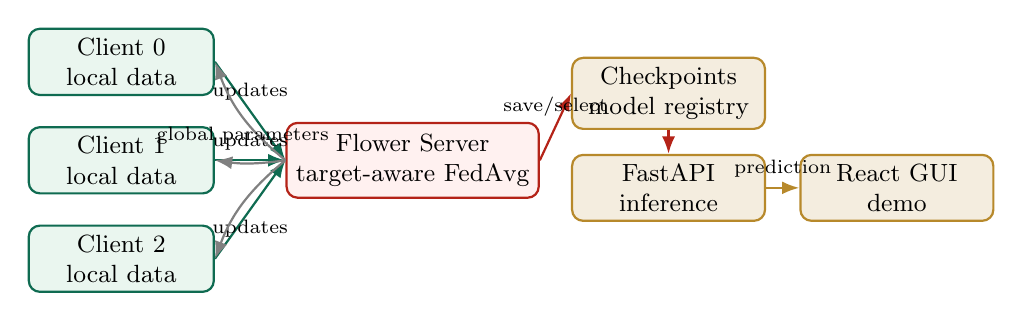
\begin{tikzpicture}[
    node distance=0.8cm,
    client/.style={rectangle, rounded corners, draw=bankgreen, fill=softgreen, thick, align=center, minimum width=2.35cm, minimum height=0.78cm, font=\small},
    server/.style={rectangle, rounded corners, draw=bankred, fill=softred, thick, align=center, minimum width=2.95cm, minimum height=0.95cm, font=\small},
    api/.style={rectangle, rounded corners, draw=bankgold, fill=bankgold!15, thick, align=center, minimum width=2.45cm, minimum height=0.82cm, font=\small},
    arrow/.style={-{Latex[length=2.2mm]}, thick}
  ]
    \node[client] (c0) at (0,1.25) {Client 0\\local data};
    \node[client] (c1) at (0,0) {Client 1\\local data};
    \node[client] (c2) at (0,-1.25) {Client 2\\local data};
    \node[server] (server) at (3.7,0) {Flower Server\\target-aware FedAvg};
    \node[api] (ckpt) at (6.95,0.85) {Checkpoints\\model registry};
    \node[api] (api) at (6.95,-0.35) {FastAPI\\inference};
    \node[api] (gui) at (9.85,-0.35) {React GUI\\demo};

    \draw[arrow, draw=bankgreen] (c0.east) -- node[above,font=\scriptsize]{updates} (server.west);
    \draw[arrow, draw=bankgreen] (c1.east) -- node[above,font=\scriptsize]{updates} (server.west);
    \draw[arrow, draw=bankgreen] (c2.east) -- node[below,font=\scriptsize]{updates} (server.west);

    \draw[arrow, draw=gray] (server.west) to[bend left=15] node[below,font=\scriptsize]{global parameters} (c0.east);
    \draw[arrow, draw=gray] (server.west) to[bend left=8] (c1.east);
    \draw[arrow, draw=gray] (server.west) to[bend right=15] (c2.east);

    \draw[arrow, draw=bankred] (server.east) -- node[above,font=\scriptsize]{save/select} (ckpt.west);
    \draw[arrow, draw=bankred] (ckpt.south) -- (api.north);
    \draw[arrow, draw=bankgold] (api.east) -- node[above,font=\scriptsize]{prediction} (gui.west);
  \end{tikzpicture}
  \vspace{0.25cm}
  \begin{block}{Core distributed point}
    Raw transaction rows stay on clients. Only model updates, checkpoints, metrics, and prediction requests move.
  \end{block}
\end{frame}

\begin{frame}{Base FedAvg}
  Each client trains locally and returns parameters \(\theta_i\).
  \[
    \theta_{t+1}
    =
    \sum_{i=1}^{K}
    \frac{n_i}{\sum_{j=1}^{K} n_j}
    \theta_i
  \]
  \footnotesize \(K\): number of clients \quad \(\theta_i\): client \(i\)'s trained parameters \quad \(n_i\): client \(i\)'s row count \quad \(\theta_{t+1}\): new global parameters
  \normalsize
  \begin{block}{Meaning}
    Larger clients contribute more because they have more training rows.
  \end{block}
  \begin{block}{Limitation}
    In fraud detection, a smaller or harder client may matter more because missing fraud on that client is costly.
  \end{block}
\end{frame}

\begin{frame}{Target-Aware Weighted Aggregation}
  \[
  \operatorname{target\_score}_i =
  0.35 \min\left(\frac{\operatorname{AUPRC}_i}{0.70},1\right)
  + 0.20 \min\left(\frac{\operatorname{AUROC}_i}{0.90},1\right)
  + 0.45 \min\left(\frac{F1_i}{0.70},1\right)
  \]
  \[
    q_i = 1 + 0.15(1-\min(\operatorname{target\_score}_i,1))
  \]
  \[
    a_i = q_i\sqrt{n_i}
    \qquad
    w_i = \frac{a_i}{\sum_j a_j}
    \qquad
    \theta_{t+1} = \sum_i w_i\theta_i
  \]
  \footnotesize \(\operatorname{AUPRC}_i,\operatorname{AUROC}_i,F1_i\): client \(i\)'s validation metrics \quad \(q_i\): quality multiplier (\(>1\) for under-target clients) \quad \(a_i\): quality-adjusted weight \quad \(w_i\): final normalized aggregation weight
  \normalsize
  \begin{block}{Presentation line}
    This is still FedAvg, but it gives extra attention to clients below target so the global model does not ignore weak clients.
  \end{block}
\end{frame}

\section{Results and Demo}

\begin{frame}{Best Checkpoint Result}
  \begin{columns}[T]
    \begin{column}{0.58\textwidth}
      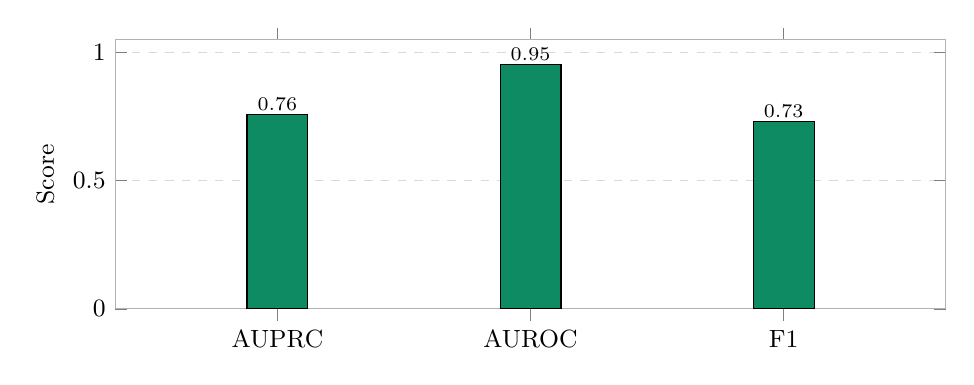
\begin{tikzpicture}
        \begin{axis}[
          ybar,
          width=\textwidth,
          height=5.0cm,
          ymin=0,
          ymax=1.05,
          ylabel={Score},
          symbolic x coords={AUPRC,AUROC,F1},
          xtick=data,
          nodes near coords={\pgfmathprintnumber[fixed,precision=2]{\pgfplotspointmeta}},
          every node near coord/.append style={font=\scriptsize, yshift=-2pt},
          bar width=22pt,
          enlarge x limits=0.32,
          ymajorgrids=true,
          grid style={dashed,gray!30},
          axis line style={gray!60},
          tick label style={font=\small},
          label style={font=\small}
        ]
          \addplot[fill=bankgreen2] coordinates {(AUPRC,0.7593) (AUROC,0.9525) (F1,0.7303)};
        \end{axis}
      \end{tikzpicture}
    \end{column}
    \begin{column}{0.39\textwidth}
      \vspace{0.1cm}
      \begin{table}
        \centering
        \small
        \begin{tabular}{lrr}
          \toprule
          Metric & Target & Best \\
          \midrule
          AUPRC & 0.70 & \bestAUPRC \\
          AUROC & 0.90 & \bestAUROC \\
          F1 & 0.70 & \bestFone \\
          \bottomrule
        \end{tabular}
      \end{table}
      \vspace{-0.15cm}
      \begin{block}{Selected checkpoint}
        \small
        \texttt{target\_met\_round\_024.pt}\\
        Threshold: \(\tau=\bestThreshold\)
      \end{block}
      \small
      All three core targets are above the required line.
    \end{column}
  \end{columns}
\end{frame}

\begin{frame}{Why the GUI Chooses Round 24}
  \begin{block}{Selection rule}
    The GUI does not blindly select the newest checkpoint. It ranks checkpoints by validation quality, target status, worst-client behavior, loss, and stability.
  \end{block}
  \begin{columns}[T]
    \begin{column}{0.48\textwidth}
      \textbf{Best ranked checkpoint}
      \begin{itemize}
        \item \texttt{target\_met\_round\_024.pt}
        \item AUPRC = 0.7593
        \item AUROC = 0.9525
        \item F1 = 0.7303
      \end{itemize}
    \end{column}
    \begin{column}{0.48\textwidth}
      \textbf{Later rounds}
      \begin{itemize}
        \item Still meet the core target
        \item Show plateau or stalling
        \item Lower stability/ranking score
      \end{itemize}
    \end{column}
  \end{columns}
\end{frame}

\begin{frame}{Demo Flow}
  \centering
  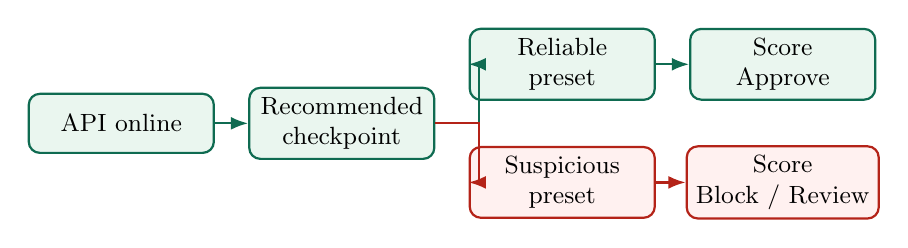
\begin{tikzpicture}[
    node distance=0.75cm,
    box/.style={rectangle, rounded corners, draw=bankgreen, fill=softgreen, thick, align=center, minimum width=2.35cm, minimum height=0.75cm, font=\small},
    boxr/.style={rectangle, rounded corners, draw=bankred, fill=softred, thick, align=center, minimum width=2.35cm, minimum height=0.75cm, font=\small},
    arrow/.style={-{Latex[length=2.2mm]}, thick}
  ]
    \node[box] (api) at (0,0.9) {API online};
    \node[box] (model) at (2.8,0.9) {Recommended\\checkpoint};
    \node[box] (reliable) at (5.6,1.65) {Reliable\\preset};
    \node[box] (score1) at (8.4,1.65) {Score\\Approve};
    \node[boxr] (suspicious) at (5.6,0.15) {Suspicious\\preset};
    \node[boxr] (score2) at (8.4,0.15) {Score\\Block / Review};

    \draw[arrow, draw=bankgreen] (api) -- (model);
    \draw[arrow, draw=bankgreen] (model.east) -- ++(0.55,0) |- (reliable.west);
    \draw[arrow, draw=bankred] (model.east) -- ++(0.55,0) |- (suspicious.west);
    \draw[arrow, draw=bankgreen] (reliable) -- (score1);
    \draw[arrow, draw=bankred] (suspicious) -- (score2);
  \end{tikzpicture}
  \vspace{0.4cm}
  \begin{block}{What the demo proves}
    Same model and same API endpoint. The decision changes because the feature vector changes.
  \end{block}
\end{frame}

\begin{frame}[fragile]{Live Demo Commands}
  Start the FastAPI inference gateway:
  \begin{verbatim}
uv run uvicorn api.main:app --host 127.0.0.1 --port 8000
  \end{verbatim}
  Start the React GUI:
  \begin{verbatim}
cd app
npm run dev -- --host 127.0.0.1 --port 5173
  \end{verbatim}
  Open:
  \begin{verbatim}
http://127.0.0.1:5173
  \end{verbatim}
  \begin{block}{What to say}
    The GUI calls FastAPI, FastAPI loads the selected PyTorch checkpoint, and the backend reconstructs the same schema used during training.
  \end{block}
\end{frame}

\begin{frame}{Reliable vs Suspicious Signals}
  \begin{columns}[T]
    \begin{column}{0.48\textwidth}
      \begin{block}{Reliable preset}
        \begin{itemize}
          \item Low amount
          \item Daytime transaction
          \item Matched email/domain
          \item Established account age
          \item Low recent transaction count
          \item Clean backward-looking history
        \end{itemize}
      \end{block}
    \end{column}
    \begin{column}{0.48\textwidth}
      \begin{alertblock}{Suspicious preset}
        \begin{itemize}
          \item High amount
          \item Late hour
          \item Email mismatch
          \item New account
          \item High velocity/distance
          \item Prior fraud and chargebacks
        \end{itemize}
      \end{alertblock}
    \end{column}
  \end{columns}
  \begin{block}{Safe wording}
    One field alone does not prove fraud. Risk increases when several abnormal signals appear together.
  \end{block}
\end{frame}

\begin{frame}{Why More Money Can Lower the Score}
  \begin{block}{Not a rule-based model}
    Amount alone is not monotonic. A high amount with normal identity and clean history can still look legitimate.
  \end{block}
  The model score uses:
  \[
    p = \sigma(f(x_1,x_2,\ldots,x_{316}))
  \]
  \begin{itemize}
    \item Amount is transformed, normalized, and combined with other features.
    \item Normal timing, matched identity, clean history, and low velocity can push the score down.
    \item Suspicious preset changes multiple signals together, so the score rises.
  \end{itemize}
\end{frame}

\section{Fault Tolerance and Scalability}

\begin{frame}{Checkpoint and Recovery Algorithm}
  \begin{columns}[T]
    \begin{column}{0.48\textwidth}
      At round \(r\), after aggregation:
      \[
        C_r = (r,\theta_r,\operatorname{metadata}_r)
      \]
      Save:
      \[
        C_r \rightarrow \texttt{outputs/checkpoints/round\_r.pt}
      \]
    \end{column}
    \begin{column}{0.48\textwidth}
      On restart:
      \[
        r^* = \max\{r \mid C_r \text{ exists and compatible}\}
      \]
      \[
        \theta_{\text{start}} = \theta_{r^*}
      \]
      Continue training from \(\theta_{\text{start}}\).
    \end{column}
  \end{columns}
  \begin{block}{Evidence in code}
    \texttt{src/server/checkpoint\_manager.py}, \texttt{scripts/run\_server.py}, drift rollback tests.
  \end{block}
  \footnotesize \(r\): round number \quad \(\theta_r\): global parameters at round \(r\) \quad \(C_r\): saved checkpoint (round, parameters, metadata) \quad \(r^*\): most recent usable checkpoint round
\end{frame}

\begin{frame}{Round-Level Fault Tolerance}
  Successful clients in round \(t\):
  \[
    S_t = \{i \mid \text{client } i \text{ returned update before timeout}\}
  \]
  Commit rule:
  \[
    \text{if } |S_t| \geq 2:
    \quad
    \theta_{t+1} = \sum_{i\in S_t} w_i\theta_i
  \]
  \[
    \text{else: no new checkpoint is committed}
  \]
  \footnotesize \(S_t\): clients that responded on time in round \(t\) \quad \(w_i\): client \(i\)'s aggregation weight
  \normalsize
  \begin{block}{Interpretation}
    Failed clients are excluded from the current aggregation. The previous checkpoint remains the recoverable state.
  \end{block}
\end{frame}

\begin{frame}{Phi Accrual Failure Detector Extension}
  Heartbeat interval:
  \[
    \Delta_k = \operatorname{heartbeat}_k - \operatorname{heartbeat}_{k-1}
  \]
  Estimate distribution \(F(\Delta)\) from recent intervals.
  \[
    \phi(t) =
    -\log_{10}\left(1 - F(t - t_{\text{last}})\right)
  \]
  Decision:
  \[
    \phi(t)\geq 8 \Rightarrow \text{suspect client}
  \]
  \footnotesize \(\Delta_k\): gap between consecutive heartbeats \quad \(F(\Delta)\): observed distribution of those gaps \quad \(\phi(t)\): suspicion level given silence since \(t_{\text{last}}\)
  \normalsize
  \begin{block}{Presentation line}
    Current implementation uses Flower round-level failures. Phi Accrual or SWIM is the production extension for adaptive membership detection.
  \end{block}
\end{frame}

\begin{frame}{Scalability: Communication Cost}
  Model-update communication:
  \[
    \operatorname{cost}_{FL} = O(KP) + O(KM)
  \]
  \[
    K=\text{clients},\quad P=\text{model parameters},\quad M=\text{scalar metrics}
  \]
  Central raw-data communication:
  \[
    \operatorname{cost}_{centralized}
    =
    O(\text{rows}\times\text{features})
  \]
  \begin{block}{Why this scales better}
    Raw transaction rows stay local. Only model parameters and compact metrics move over the network.
  \end{block}
\end{frame}

\section{Q\&A Support}

\begin{frame}{Q\&A: Worker Failure and Reassignment}
  This project is fraud detection, but the distributed task principle maps to password cracking.
  \[
    K = \{0,1,\ldots,N-1\}
  \]
  Partition into chunks:
  \[
    C_j = [a_j,b_j)
  \]
  Lease assignment:
  \[
    \operatorname{state}(C_j)=\operatorname{leased},
    \quad
    \operatorname{owner}(C_j)=w,
    \quad
    \operatorname{lease\_expiry}(C_j)=\operatorname{now}+TTL
  \]
  Recovery:
  \[
    \operatorname{now}>\operatorname{lease\_expiry}(C_j)
    \Rightarrow C_j \text{ becomes unassigned}
  \]
  \footnotesize \(K\): the full keyspace, split into chunks \(C_j=[a_j,b_j)\) \quad \(w\): the worker currently leasing a chunk \quad \(TTL\): how long a lease is valid before it can be reclaimed
\end{frame}

\begin{frame}{Q\&A: Verifying a Worker Result}
  Password result verification:
  \[
    \text{accept candidate } x
    \quad \text{iff} \quad
    h(x)=H^*
  \]
  Robust federated aggregation extensions:
  \[
    \theta_{t+1}[k] = \operatorname{median}_i(\theta_i[k])
  \]
  Trimmed mean:
  \[
    \theta_{t+1}[k]
    =
    \operatorname{mean}(\text{middle values after removing largest and smallest } f)
  \]
  Norm clipping:
  \[
    \Delta_i^{clip}
    =
    \Delta_i \cdot \min\left(1,\frac{C}{\|\Delta_i\|_2}\right)
  \]
  \footnotesize \(h(x){=}H^*\): candidate hash matches the target hash \quad \(\theta_i[k]\): client \(i\)'s value for parameter \(k\) \quad \(f\): fraction trimmed from each end \quad \(\Delta_i\): client \(i\)'s update, capped to norm \(C\)
\end{frame}

\begin{frame}{Q\&A: Telemetry Without Network Slowdown}
  Send compact telemetry occasionally:
  \[
    m_i(t)=
    [
      \text{cpu mean},
      \text{cpu p95},
      \text{memory used},
      \text{GPU memory},
      \text{train time},
      \text{batch size}
    ]
  \]
  Quantization:
  \[
    q = \operatorname{round}\left(\frac{\text{value}}{\text{scale}}\right)
  \]
  Rate limiting:
  \[
    \text{send only every } R \text{ rounds or when } |\Delta|>\epsilon
  \]
  \footnotesize \(q\): quantized (rounded) telemetry value \quad \(R\): reporting interval in rounds \quad \(\epsilon\): minimum change needed to trigger an early report
  \normalsize
  \begin{block}{Network cost}
    Telemetry cost is \(O(KM)\), tiny compared with model parameter transfer.
  \end{block}
\end{frame}

\begin{frame}{Future Work and Paper Extension}
  \begin{block}{Extension over FedAvg}
    Target-aware and fairness-aware aggregation for fraud detection.
  \end{block}
  \begin{itemize}
    \item Downweight unstable or suspicious updates.
    \item Prioritize clients with high drift or low AUPRC.
    \item Add Phi/SWIM membership for faster failure detection.
    \item Use replicated checkpoint metadata with Raft for high availability.
    \item Add robust aggregation for Byzantine or fake updates.
  \end{itemize}
\end{frame}

\begin{frame}{Closing}
  \begin{block}{Summary}
    The project is a complete federated fraud detection pipeline:
    preprocessing, feature engineering, client training, server aggregation,
    checkpoint recovery, drift rollback, API inference, and GUI demonstration.
  \end{block}
  \begin{block}{Result}
    Core target is met: AUPRC \(=\bestAUPRC\), AUROC \(=\bestAUROC\), F1 \(=\bestFone\).
  \end{block}
  \begin{block}{Final line}
    Raw data stays local, the model improves globally, and the system can be demonstrated end to end.
  \end{block}
\end{frame}

\begin{frame}{Sources: Core Project}
  \small
  \begin{tabular}{p{0.28\textwidth}p{0.64\textwidth}}
    \toprule
    Topic & Source and purpose \\
    \midrule
    Federated learning &
    McMahan et al. \textit{Communication-Efficient Learning of Deep Networks from Decentralized Data}. Base FedAvg rule. \url{https://arxiv.org/abs/1602.05629} \\
    Flower implementation &
    Flower FedAvg documentation. Framework reference for server aggregation. \url{https://flower.ai/docs/framework/ref-api/flwr.serverapp.strategy.FedAvg.html} \\
    Dataset &
    IEEE-CIS Fraud Detection. Source dataset for transaction fraud. \url{https://www.kaggle.com/competitions/ieee-fraud-detection} \\
    Residual model idea &
    He et al. \textit{Deep Residual Learning for Image Recognition}. Residual block inspiration. \url{https://arxiv.org/abs/1512.03385} \\
    Normalization layer &
    Ba, Kiros, Hinton. \textit{Layer Normalization}. LayerNorm head. \url{https://arxiv.org/abs/1607.06450} \\
    \bottomrule
  \end{tabular}
\end{frame}

\begin{frame}{Sources: Metrics and Q\&A Extensions}
  \small
  \begin{tabular}{p{0.28\textwidth}p{0.64\textwidth}}
    \toprule
    Topic & Source and purpose \\
    \midrule
    Precision-recall metrics &
    Davis and Goadrich. \textit{The Relationship Between Precision-Recall and ROC Curves}. Why AUPRC matters under class imbalance. \\
    High-cardinality history &
    Micci-Barreca. \textit{A Preprocessing Scheme for High-Cardinality Categorical Attributes}. Supports smoothed historical fraud-rate idea. \\
    Phi failure detector &
    Hayashibara et al. \textit{The \(\phi\) Accrual Failure Detector}. Adaptive failure suspicion. \\
    SWIM membership &
    Das, Gupta, Motivala. \textit{SWIM}. Scalable membership and failure detection. \\
    Raft consensus &
    Ongaro and Ousterhout. \textit{In Search of an Understandable Consensus Algorithm}. Replicated checkpoint metadata extension. \\
    Robust aggregation &
    Byzantine-resilient aggregation references: Krum, coordinate median, trimmed mean, and norm clipping. \\
    \bottomrule
  \end{tabular}
\end{frame}

\end{document}
